% CVPR 2024 Paper Template; see https://github.com/cvpr-org/author-kit

\documentclass[10pt,twocolumn,letterpaper]{article}

%%%%%%%%% PAPER TYPE  - PLEASE UPDATE FOR FINAL VERSION
% \usepackage{cvpr}              % To produce the CAMERA-READY version
\usepackage[review]{cvpr}      % To produce the REVIEW version
% \usepackage[pagenumbers]{cvpr} % To force page numbers, e.g. for an arXiv version

% Import additional packages in the preamble file, before hyperref
%
% --- inline annotations
%
\usepackage[dvipsnames]{xcolor}
\newcommand{\red}[1]{{\color{red}#1}}
\newcommand{\todo}[1]{{\color{red}#1}}
\newcommand{\TODO}[1]{\textbf{\color{red}[TODO: #1]}}
% --- disable by uncommenting  
% \renewcommand{\TODO}[1]{}
% \renewcommand{\todo}[1]{#1}



% It is strongly recommended to use hyperref, especially for the review version.
% hyperref with option pagebackref eases the reviewers' job.
% Please disable hyperref *only* if you encounter grave issues, 
% e.g. with the file validation for the camera-ready version.
%
% If you comment hyperref and then uncomment it, you should delete *.aux before re-running LaTeX.
% (Or just hit 'q' on the first LaTeX run, let it finish, and you should be clear).
\definecolor{cvprblue}{rgb}{0.21,0.49,0.74}
\usepackage[pagebackref,breaklinks,colorlinks,citecolor=cvprblue]{hyperref}

%%%%%%%%% PAPER ID  - PLEASE UPDATE
\def\paperID{*****} % *** Enter the Paper ID here
\def\confName{CVPR}
\def\confYear{2024}

%%%%%%%%% TITLE - PLEASE UPDATE
\title{\LaTeX\ Author Guidelines for \confName~Proceedings}

%%%%%%%%% AUTHORS - PLEASE UPDATE
\author{First Author\\
Institution1\\
Institution1 address\\
{\tt\small firstauthor@i1.org}
% For a paper whose authors are all at the same institution,
% omit the following lines up until the closing ``}''.
% Additional authors and addresses can be added with ``\and'',
% just like the second author.
% To save space, use either the email address or home page, not both
\and
Second Author\\
Institution2\\
First line of institution2 address\\
{\tt\small secondauthor@i2.org}
}

\begin{document}
\maketitle
\begin{abstract}
 Current monocular 3D scene reconstruction (3DR) works are either fully-supervised, or not generalizable, or implicit in 3D representation. We propose a novel framework - \textbf{MonoSelfRecon} that for the first time achieves \textbf{explicit 3D mesh} reconstruction for \textbf{generalizable} indoor scenes with monocular RGB views by purely \textbf{self-supervision} on voxel-SDF (signed distance function). MonoSelfRecon follows an Autoencoder-based architecture, decodes voxel-SDF and a generalizable Neural Radiance Field (NeRF), which is used to guide voxel-SDF in self-supervision. We propose novel self-supervised losses, which not only support pure self-supervision, but can be used together with supervised signals to further boost supervised training. Our experiments show that "MonoSelfRecon" trained in pure self-supervision outperforms current best self-supervised indoor depth estimation models and is comparable to 3DR models trained in fully supervision with depth annotations. MonoSelfRecon is not restricted by specific model design, which can be used to any models with voxel-SDF for purely self-supervised manner. %\footnote{Datasets  were  downloaded  and  evaluated  solely  by  the researchers from UC San Diego.}
\end{abstract}    
\section{Introduction} \label{intro}


With the recent development of deep generative models, speech synthesis has seen an extraordinary progress. Among the conventional speech synthesis methods, WaveNets~\cite{oord2016wavenet} were demonstrated to generate high-fidelity audio samples in an autoregressive manner yet suffering from prohibitively expensive computational costs. In contrast, non-autoregressive approaches such as flow-based and GAN-based models~\cite{prenger2019waveglow,jang2021univnet,kong2020hifi,huang2021multi} were also proposed to generate speech audios with satisfactory speed. However, these models were still criticized for other problems, e.g., the limited sample quality or sample diversity \cite{xiao2021tackling}.

In speech synthesis, our goal is mainly two-fold:
\begin{itemize}
    \item High-quality: generating high-quality speech is a challenging problem especially when the sampling rate of an audio is high. It is vital to reconstruct details at different timescales for waveforms of highly variable patterns.
    \item Fast: high generation speed is essential when considering real-time speech synthesis. This poses a challenge for all high-quality neural synthesizers.
\end{itemize}

As a blossoming class of generative models, denoising diffusion probabilistic models (DDPMs)~\cite{ho2020denoising,song2020denoising,lam2022bddm,liu2022pseudo} has emerged to prove its capability to achieve leading performances in both image and audio syntheses~\cite{dhariwal2021diffusion,san2021noise,kong2020diffwave,chen2020wavegrad,lam2022bddm}. However, current development of DDPMs in speech synthesis was hampered by two major challenges:
\begin{itemize}
\item Different from other existing generative models, diffusion models are not trained to directly minimize the difference between the generated audio and the reference audio, but to de-noise a noisy sample given an optimal gradient. This in practice could lead to overly de-noised speech after a large number of sampling steps, in which natural voice characteristics including breathiness and vocal fold closure are removed.
\item While DDPMs inherently are gradient-based models, a guarantee of high sample quality typically comes at a cost of hundreds to thousands of de-noising steps. When reducing the sampling steps, an apparent degradation in quality due to perceivable background noise is observed.
\end{itemize}

In this work, we propose FastDiff, a fast conditional diffusion model for high-quality speech synthesis. To improve audio quality, FastDiff adopts a stack of time-aware location-variable convolutions of diverse receptive field patterns to efficiently model long-term time dependencies with adaptive conditions. To accelerate the inference procedure, FastDiff also includes a noise schedule predictor, which derives a short and effective noise schedule and significantly reduces the de-noising steps. Based on FastDiff, we also introduce an end-to-end phoneme-to-waveform synthesizer FastDiff-TTS, which simplifies the text-to-speech generation pipeline and does not require intermediate features or specialized loss functions to enjoy low inference latency.

Experimental results demonstrated that FastDiff achieved a higher MOS score than the best publicly available models and outperformed the strong WaveNet vocoder (MOS: 4.28 vs. 4.20). FastDiff further enjoys an effective sampling process and only needs 4 iterations to synthesize high-fidelity speech, 58x faster than real-time on a V100 GPU without engineered kernels. To the best of our knowledge, FastDiff is the first diffusion model with a sampling speed comparable to previous  for the first time applicable to interactive, real-world speech synthesis applications at a low computational cost. FastDiff-TTS successfully simplify the text-to-speech generation pipeline and outperform competing architectures.
\input{sec/2_formatting}
\input{sec/3_finalcopy}
{
    \small
    \bibliographystyle{ieeenat_fullname}
    \bibliography{main}
}

% WARNING: do not forget to delete the supplementary pages from your submission 
% \clearpage
\setcounter{page}{1}
\maketitlesupplementary


\section{Relationship with MonoNeRF \cite{mononerf}}
\label{sec:relationship with mononerf}
We discuss the relationship between our strongest baseline MonoNeRF\cite{mononerf} and our proposed method MonoSelfRecon as follows: 1) We share the same idea of SFM-based 3DR with monocular RGB sequence as input, and we both jointly train SFM and a generalizable NeRF, where the NeRF is used to boost SFM performance.  2) Although using SFM as the core of framework design, we regress to different 3D representations, where MonoNeRF regress to view-based 2D depth map while we regress to 3D voxel-based SDF values. 3) While MonoNeRF also jointly estimates camera poses, their 2D view-based depth representation restricts the ability to incrementally complete a whole scene in 3D mesh representation. Fusing TSDF from direct depth estimation is time-consuming, and will cause layered or sparse mesh due to depth inconsistency between each frame. By comparison, our direct voxel-SDF regression enables us to incrementally add the previous mesh to complete the whole scene consistently in mesh representation.  

The mesh representation is a stricter 3D representation over 2D depth map. Theoretically, the depth map can be perfectly rendered from 3D mesh but cannot in reverse, which is further validated by our experiments. Table \ref{table:scannet} and \ref{table:7scenes} show that although all using ground truth for supervised training, the one that directly regresses SDF (NeuralRecon) has a clear advantage on 2D depth metrics over other supervised methods that regresses depth. The reason that although both our method and MonoNeRF are based on SFM while ours outperforms theirs can be also partly attributed to this different 3D representation. Our visual results also reflect this point in Table \ref{fig:visual results}, where although there is no much difference of 2D depth, the difference of 3D mesh is clear. In other words, the depth representation is more visually straightforward than 3D mesh. Consequently, our 3D mesh regressing is a stricter 3D geometric representation than MonoNeRF's 2D depth.


\section{Evaluation Metrics}
We follow the same evaluation metrics as \cite{atlas, neucon}. Details of the metrics are summarized in Table \ref{table:metrics}.
\begin{table}[htb]
\tiny
\setlength\tabcolsep{0.1pt}
\begin{tabular*}{\columnwidth}{@{\extracolsep{\fill}} llll}
\hline
\multicolumn{2}{l}{2D} & \multicolumn{2}{l}{3D} \\ \hline
Abs Rel             & $\frac{1}{n}\sum\left|d-d^*\right|/d^*$      & Acc       & $\text{mean}_{p \in P}\left(\min_{p^* \in P^*}||p-p^*||\right)$\\
Abs Diff            & $\frac{1}{n}\sum\left|d-d^*\right|$          & Comp      & $\text{mean}_{p^* \in P^*}\left(\min_{p \in P}||p-p^*||\right)$\\
Sq Rel              & $\frac{1}{n}\sum\left|d-d^*\right|^2/d^*$    & Prec      & $\text{mean}_{p \in P}\left(\min_{p^* \in P^*}||p-p^*||<.05\right)$\\
RMSE                & $\sqrt{\frac{1}{n}\sum\left|d-d^*\right|^2}$ & Recal     & $\text{mean}_{p^* \in P^*}\left(\min_{p \in P}||p-p^*||<.05\right)$\\
$\tiny\mkern-5mu\sigma<1.25$   & $\frac{1}{n}\sum\left(\max\left(\frac{d}{d^*}, \frac{d^*}{d}\right)<1.25\right)$ & F-score  & $\frac{2 \times \text{Prec} \times \text{Recal}}{\text{Prec} + \text{Recal}}$\\
Comp                & \% valid predictions &                        &                 \\
RMSE log            & $\sqrt{\frac{1}{n}\sum\left|\log(d)-\log(d^*)\right|^2}$   &                        &                 \\
Sc Inv              & $\left(\frac{1}{n}\sum_{i}z_i^2-\frac{1}{n^2}(\sum_i z_i)^2\right)^{1/2}$ &                        &                 \\ \hline
\end{tabular*}
\caption{\textbf{Evaluation Metrics.}}
\label{table:metrics}
\end{table}


\section{Model Details}
\subsection{Attentional View Fusion}
We use a standard Vision Transformer (ViT) Encoder, where we keep the original high-level architecture of the ViT encoder to be: A norm layer, a multi-head attention layer, a norm layer, and a MLP (2 heads are used). Originally the ViT takes image patch/features as input, while we adopted the input to be the nearest 2D features from the projected 3D voxels, which is of size $[N_{view}, N_{points}, C]$, where $N_{view}$ is the number of views in a scene fragment, $N_{points}$ is the number of voxels in a fragment, $C$ is the feature channel. The input also takes the voxel mask as input to filter out the pixels which are invisible to the voxels, and the transformer only takes the visible pixel features. We stack two ViT encoders to update the features, where the output is still of size $[N_{view}, N_{points}, C]$. Then we use a multi-view weighted feature pooling to fuse the updated features at the view channel to 3D features of size $[N_{points}, C]$, where the weight is the number of visible views in a fragment for each voxel. Such design enables more flexibility to adjust the contribution of each view to the 3D voxels. 

\subsection{GRU}
We directly use the GRU module from \cite{neucon}, which is elaborately designed for sparse 3D convolution. The 3D voxel features are obtained by attentional view fusions and fed to the GRU module, where the current 3D fragment features are conditioned on the previous fragment. Using the current 3D global voxel features $G^l_{t}$ and the previous hidden state $H^l_{t-1}$ at layer $l$,  the current hidden state $H^l_{t}$ can be obtained, and the SDF value at each level is regressed from the hidden state $H^l_{t}$. More specifically,

\begin{equation}
\begin{aligned}
     &z_t = \sigma(SparseConv([H^{l}_{t-1}, G^l_t], W_z)) \\
     &r_t = \sigma(SparseConv([H^{l}_{t-1}, G^l_t], W_r)) \\
     &\Tilde{H^l_t} = tanh(SparseConv([r_t \odot H^l_{t-1}, G^l_t], W_h)) \\
     &H^l_t = (1-z_t)\odot H^l_{t-1} + z_{t} \odot \Tilde{H^l_t}
\end{aligned}
\end{equation}

\noindent where $z_t$ is the update gate, $r_t$ is the reset gate, $\sigma$ is the sigmoid function and $W_{*}$ is the weight for sparse convolution. 






We first train without GRU within each fragment to warmup the framework with our proposed self-supervised losses, where we call it \textbf{intra-fragment losses}. Because the GRU module is leveraged to enhance the consistency between fragments, the self-supervised learning strategy should be treated differently to intra-fragment losses. There is no need to change the training policy in purely supervised training because SDF ground truth is used, and there is no ground truth in our self-supervision except for the consistency clues between fragments. So we extend the \textbf{inter-fragment losses} to \textbf{intra-fragment losses}. While the model only takes input per fragment, backpropagating whole fragments brings memory challenges, so we only implement the inter-fragment losses on the frames around the boundary of fragments. Specifically, we use the last 4 and first 4 frames of the previous and current fragments to implement the inter-fragment loss.

\begin{figure}
    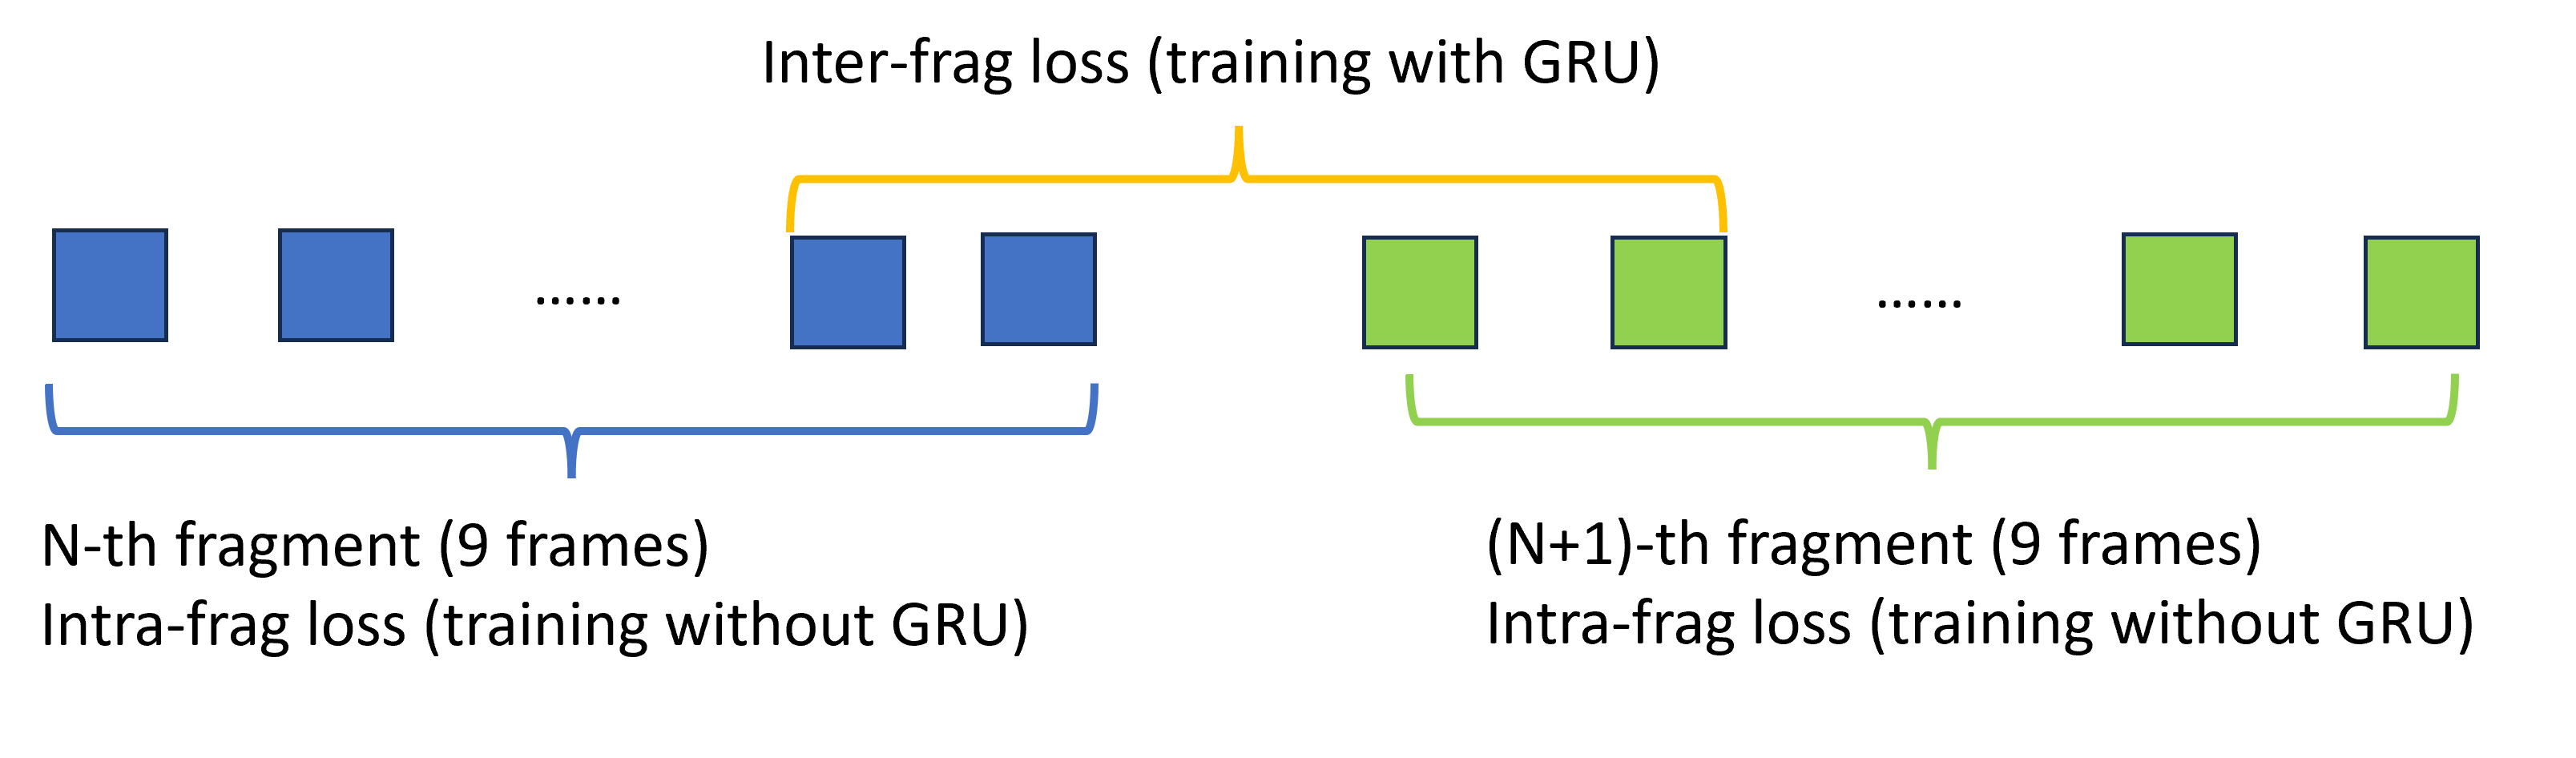
\includegraphics[width=\linewidth]{figures/GRUloss_explain.png}
    \caption{\textbf{Inter/Intra-fragment} losses illustration.}
    \label{fig:gruloss_explain}
\end{figure}


\subsection{NeRF}

\begin{figure}
    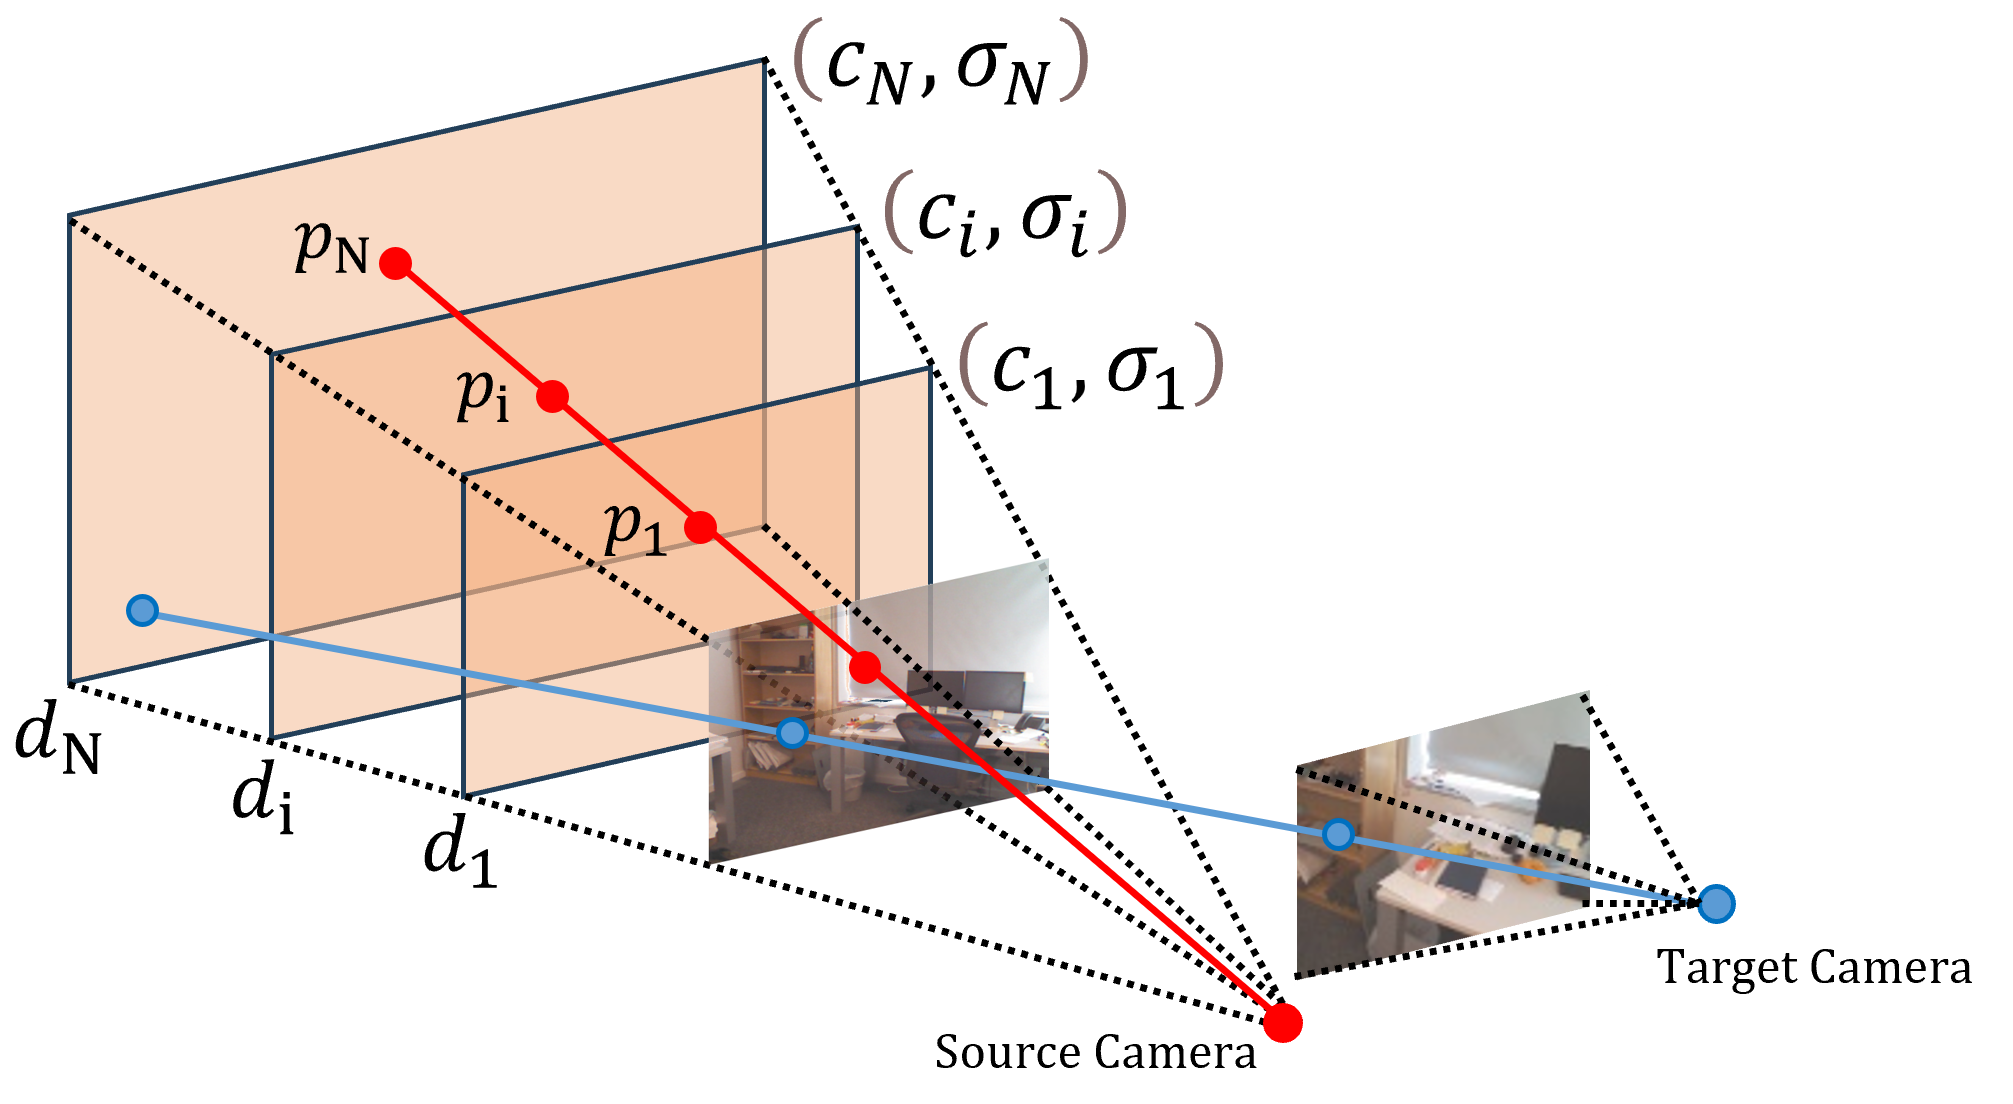
\includegraphics[width=\linewidth]{figures/MPI_explain.png}
    \caption{\textbf{Multi-Plane Image (MPI)} NeRF illustration.}
    \label{fig:mpi_explain}
\end{figure}


Since the SDF decoder is generalizable, the NeRF also must be generalizable to boost SDF decoder. For our work, we adopted MPI-NeRF\cite{mpi, mpi-nerf}, which has been directly used by MonoNeRF\cite{mononerf} and proved to be generalizable. As Figure \ref{fig:mpi_explain} shows, in Multi-Plane-Image (MPI) system, an image is represented by a set of parallel planes (orange planes) denoted as RGB-$\sigma$, specifically $(c_{i}, \sigma_{i})_{i=1}^N$,  where the $i_{th}$ plane has $d_{i}$ disparity (reverse of depth) to the camera. The shading points (red points) are selected as the intersection of the parallel planes and the rays shooting from pixels in the image, where $c_{i}$ and $\sigma_{i}$ are the RGB color and density of each shading points at $i_{th}$ plane. In a standard MPI system, the source view RGB image $\hat{I_{s}}$ and depth map $\hat{D_{}}$ can be composed using the ``over'' operation \cite{over_composite} as

\iffalse
\begin{equation}
    \Biggl\{ \begin{array}{cc}
     \hat{I}_{s} = \sum_{i=1}^{D}(c_{i}\sigma_{i}\prod_{j=i+1}^{D}(1-\sigma_{j})) \\
     \\
     \hat{D}_{s} = \sum_{i=1}^{D}(d_{i}^{-1}\sigma_{i}\prod_{j=i+1}^{D}(1-\sigma_{j}))
     \end{array}
\end{equation}
\fi


{
\begin{equation}
\begin{aligned}
    \hat{I}_s &= \sum_{i=1}^{D} (c_i \sigma_i \prod_{j=i+1}^{D} (1 - \sigma_j)) \\
    \hat{D}_s &= \sum_{i=1}^{D} (d_i^{-1} \sigma_i \prod_{j=i+1}^{D} (1 - \sigma_j))
\end{aligned}
\label{eq:combined}
\end{equation}
}

To use MPI system in NeRF style, the composition operation above can be replaced by volumetric rendering \cite{nerf} for both RGB and depth as 
\iffalse
\begin{equation}
    \Biggl\{ \begin{array}{cc}
    \hat{I_s} = \sum_{i=1}^{N}T_{i}(1-exp(-\sigma_{i}\delta_{i}))c_{i} \\
    \\
    \hat{Z_s} = \sum_{i=1}^{N}T_{i}(1-exp(-\sigma_{i}\delta_{i}))z_{i}
    \end{array}
\end{equation}
\fi

{
\begin{equation}
\begin{aligned}
    \hat{I}_s &= \sum_{i=1}^{N}T_{i}(1-exp(-\sigma_{i}\delta_{i}))c_{i} \\
    \hat{Z}_s &= \sum_{i=1}^{N}T_{i}(1-exp(-\sigma_{i}\delta_{i}))z_{i}
\end{aligned}
\label{eq:combined}
\end{equation}
}

\noindent where $z_i$ is the rendered depth (reverse of disparity) $z_i = 1/d_i$, and $\delta_i = ||p_{i+1} - p_i||_2$ is the distance between the two neighbor shading points on a ray. Then we can extend volumetric rendering to target views. First, the corresponding pixels $[u_t, v_t]$ in the target view can be found by 

\begin{equation}
    \begin{bmatrix}
        u_{s} \\
        v_{s} \\
        1
    \end{bmatrix}
    \sim K_{s}(R-tn^{T}d_{i})(K_{t})^{-1}
    \begin{bmatrix}
        u_{t} \\
        v_{t} \\
        1
    \end{bmatrix}
\end{equation}

Here, $[u_s, v_s]$ is the corresponding pixel locations in the source view, $K_s$ and $K_t$ are camera intrinsics of source and target views, $R$ and $t$ are rotation and translation from the target to source view, and $n$ is the norm vector of the $i_{th}$ plane. As the planes are parallel, the RGB $c'_i$ and density $\sigma'_i$ of shading points (blue points) on target rays (blue ray) are equal to those from source rays at the same disparity, as shown in Eq. \ref{mpinerf_samergbsigma},

\iffalse
\begin{equation}
    \Biggl\{ \begin{array}{cc}
    c_{i}'(u_{t}, v_{t}) = c_{i}(u_{s}, v_{s}) \\
    \sigma_{i}'(u_{t}, v_{t}) = \sigma_{i}(u_{s}, v_{s})
    \end{array}
    \label{mpinerf_samergbsigma}
\end{equation}
\fi

{
\begin{equation}
\begin{aligned}
    c_{i}'(u_{t}, v_{t}) = c_{i}(u_{s}, v_{s}) \\
    \sigma_{i}'(u_{t}, v_{t}) = \sigma_{i}(u_{s}, v_{s})
\end{aligned}
\label{mpinerf_samergbsigma}
\end{equation}
}

\iffalse
\begin{equation}
    \Biggl\{ \begin{array}{cc}
     \hat{I}_{t} = \sum_{i=1}^{D}(c_{i}'\sigma'_{i}\prod_{j=i+1}^{D}(1-\sigma_{j}')) \\
     \\
     \hat{D}_{t} = \sum_{i=1}^{D}(d_{i}\sigma'_{i}\prod_{j=i+1}^{D}(1-\sigma_{j}'))
     \end{array}
\end{equation}
\fi

Once we have RGB and density for target views, we can perform volumetric rendering on target views as: 
\iffalse
\begin{equation}
    \Biggl\{ \begin{array}{cc}
    \hat{I_t} = \sum_{i=1}^{N}T_{i}(1-exp(-\sigma'_{i}\delta_{i}))c'_{i} \\
    \\
    \hat{Z_t} = \sum_{i=1}^{N}T_{i}(1-exp(-\sigma'_{i}\delta_{i}))z'_{i}
    \end{array}
\end{equation}
\fi

{
\begin{equation}
\begin{aligned}
    \hat{I_t} = \sum_{i=1}^{N}T_{i}(1-exp(-\sigma'_{i}\delta_{i}))c'_{i} \\
    \hat{Z_t} = \sum_{i=1}^{N}T_{i}(1-exp(-\sigma'_{i}\delta_{i}))z'_{i}
\end{aligned}
\label{eq:combined}
\end{equation}
}

We use standard NeRF RGB loss, where $\hat{I}_s$ and $\hat{I}_t$ are self-supervised with their corresponding input images with a L1 loss. Since we directly use the reverse of disparity for depth, the depth value is scale-ambiguous. As mentioned in the paper, since there is no depth ground truth for pure self-supervision, we use SDF-depth as pseudo-depth to first recover the real scale of $\hat{Z}_s$ and $\hat{Z}_t$, then we impose a consistency loss between $\hat{Z}$ and SDF-depth to boost SDF decoder.

    

\section{Visual Results}
We show more visual results of 2D rendered depth and 3D mesh in Figure \ref{fig:scannet_supp}. \textbf{We also attach a PowerPoint file with visual results, where reviewers can rotate and zoom the 3D mesh to see the details},

\section{Limitation}
Although our work combines the advantages of ``self-supervised'' ``generalizable'' and ``3D explicit mesh'' altogether, there are still limitations. So far our MonoSelfRecon can be only used for indoor environments, because we pre-define the 3D scene fragment with a fixed voxel number. Unlike indoor 2D images where depth vary within few meters, the depth can vary significantly just within a single 2D image in outdoor. It is applicable to keep the voxel number while increasing the voxel size, but it will lead to very poor resolution within voxels, which misses most of the details. Moreover, since we regress SDF corresponding to the discrete $N\times N\times N$ voxels of scene fragment, we cannot directly estimate SDF of a continuous 3D space, unless by interpolation. By contrast, SDF-NeRF based methods estimate SDF values in continuous 3D space but it is not generalizable to another scene. Our future works will explore to make SDF-NeRF generalizable, so that the 3DR can be ``self-supervised", ``generalizable", ``explicit'', ``indoor/outdoor'', and ``continous in 3D space''. 

\newpage
\begin{figure*}
\begin{minipage}{\textwidth}
  \centerline{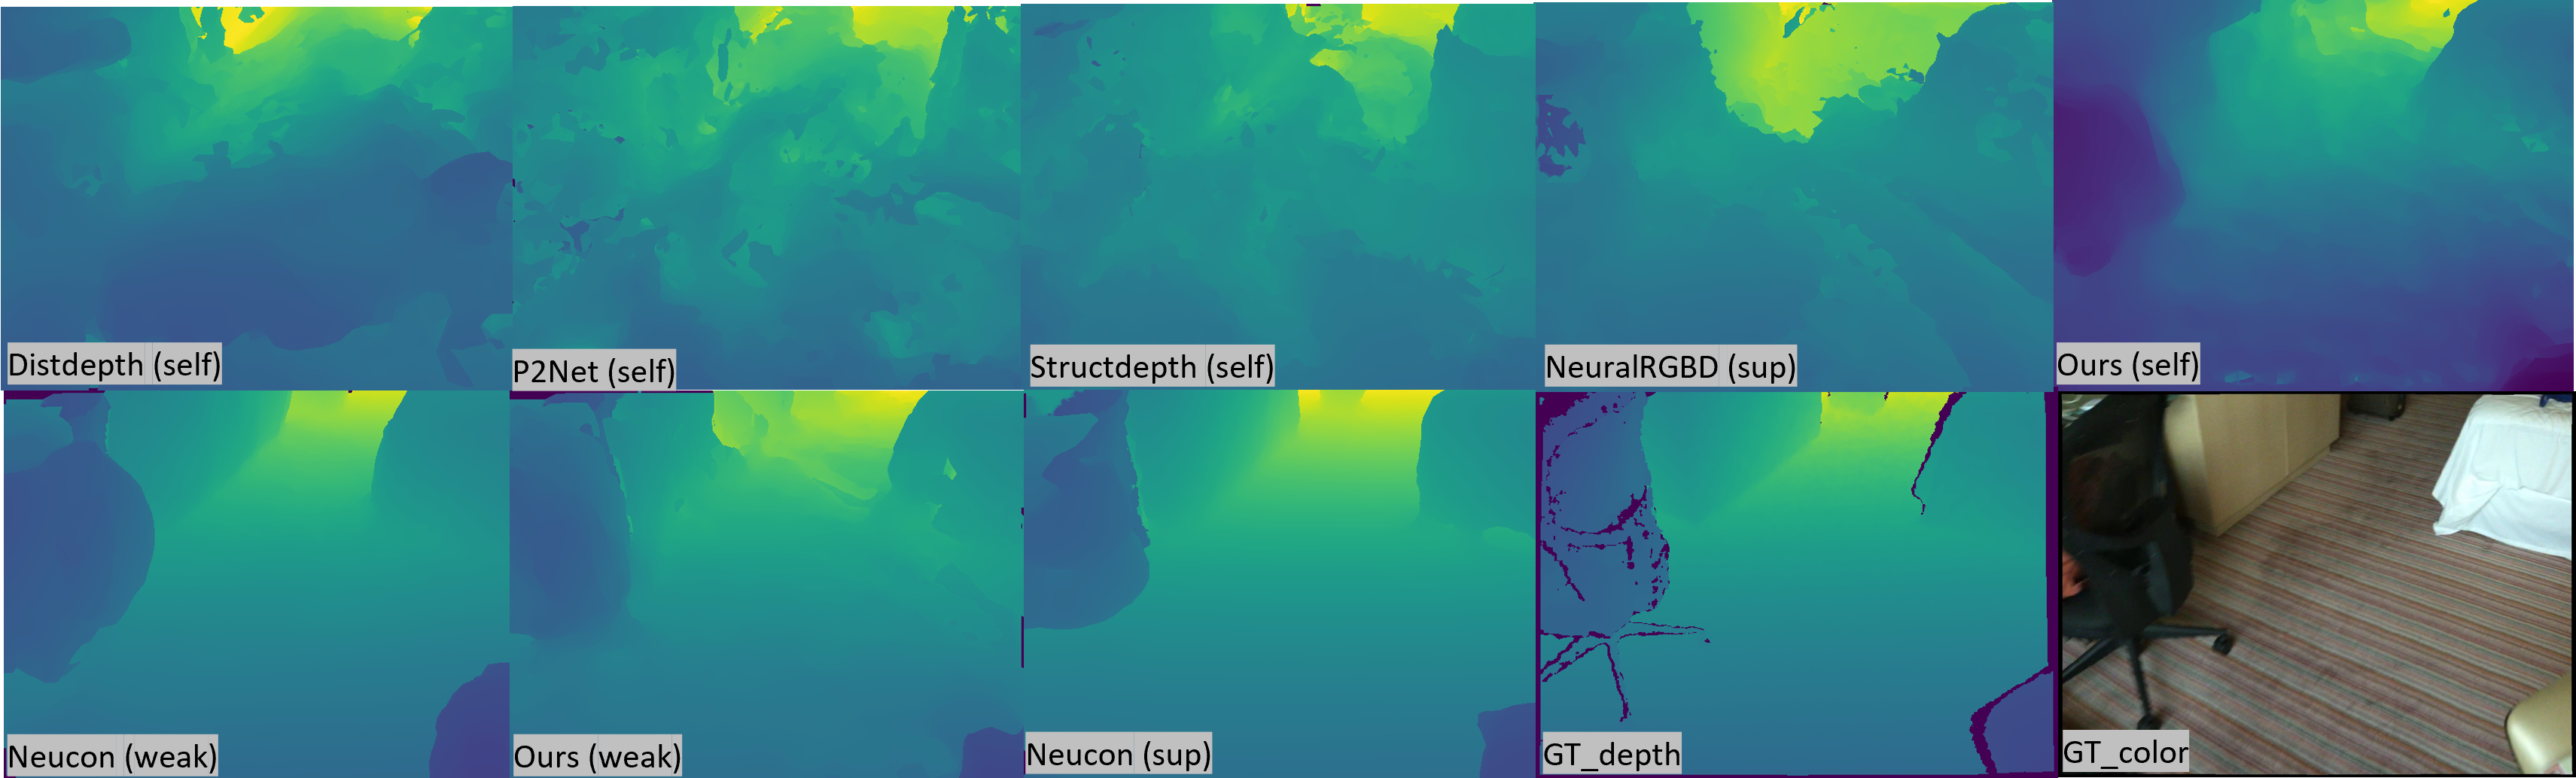
\includegraphics[width=1.0\textwidth]{figures/scannet_depth/738_1300.png}}
\end{minipage}
\vfill
\begin{minipage}{\linewidth}
  \centerline{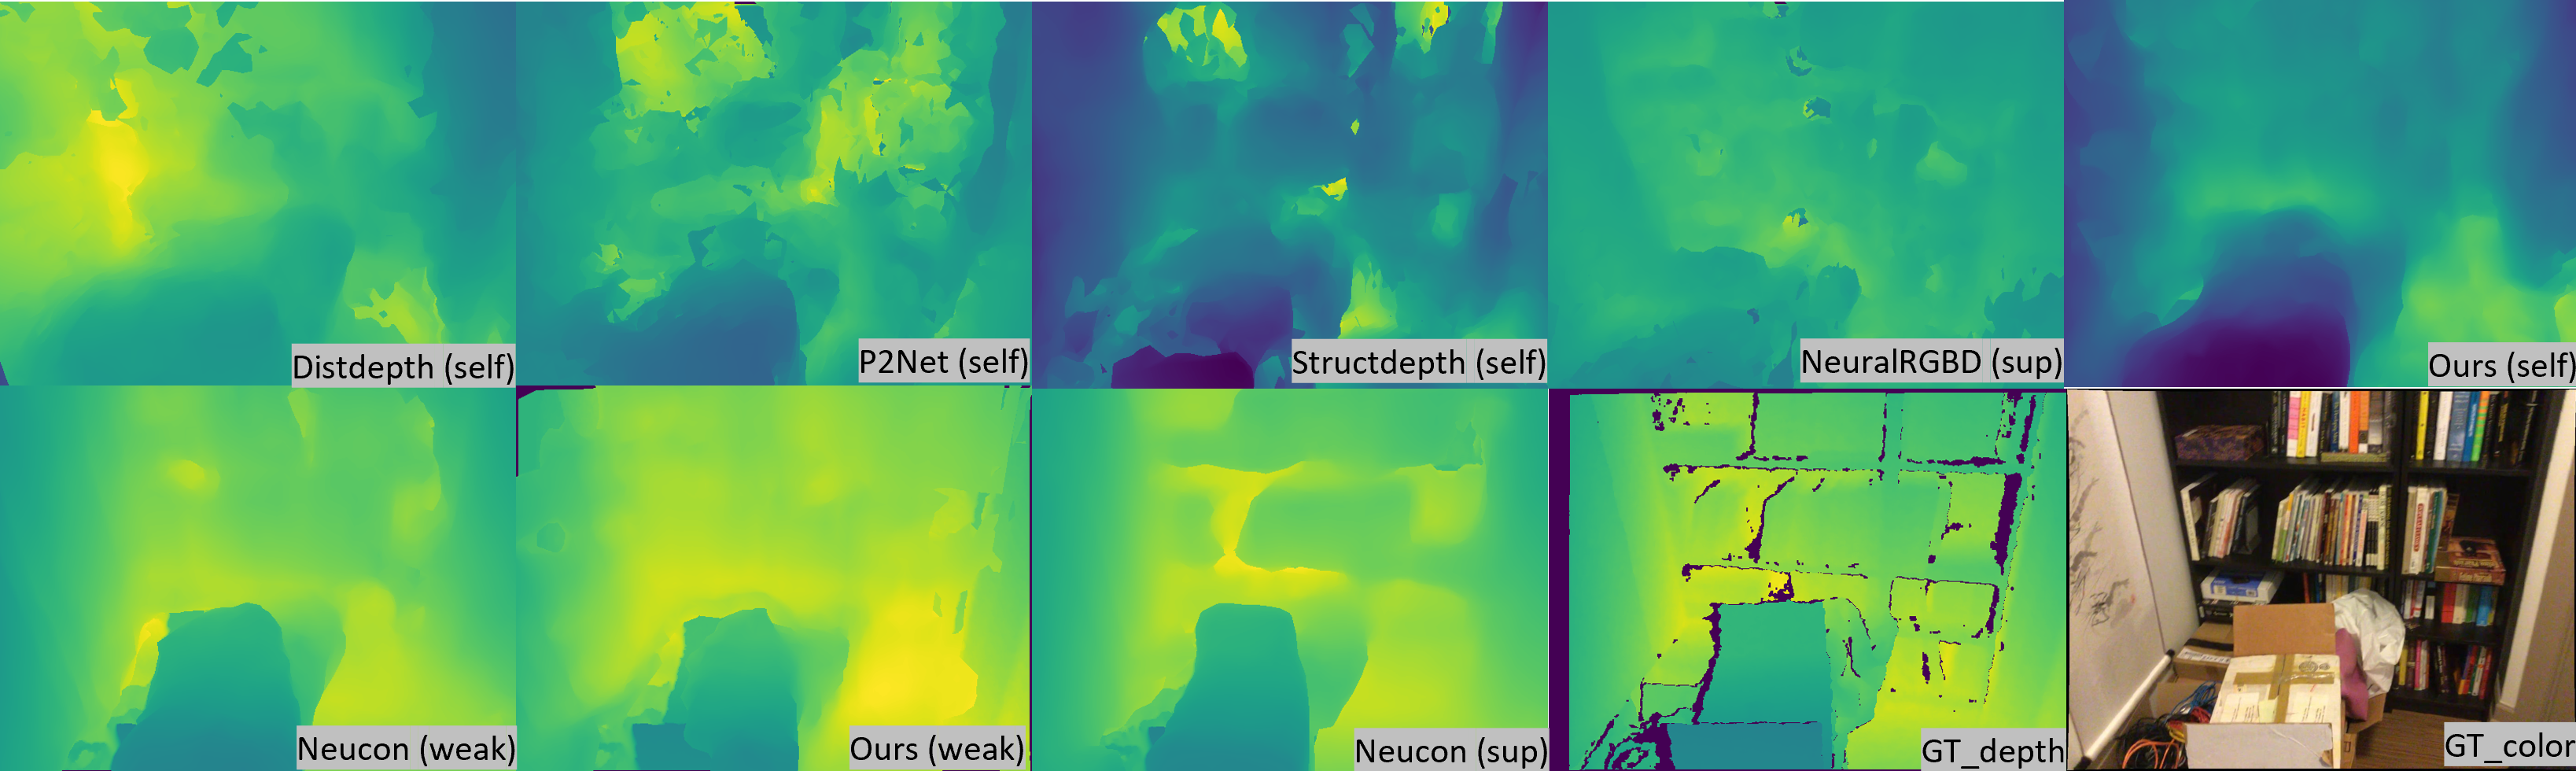
\includegraphics[width=1.0\textwidth]{figures/scannet_depth/710_1210.png}}
\end{minipage}
\vfill
\begin{minipage}{\linewidth}
  \centerline{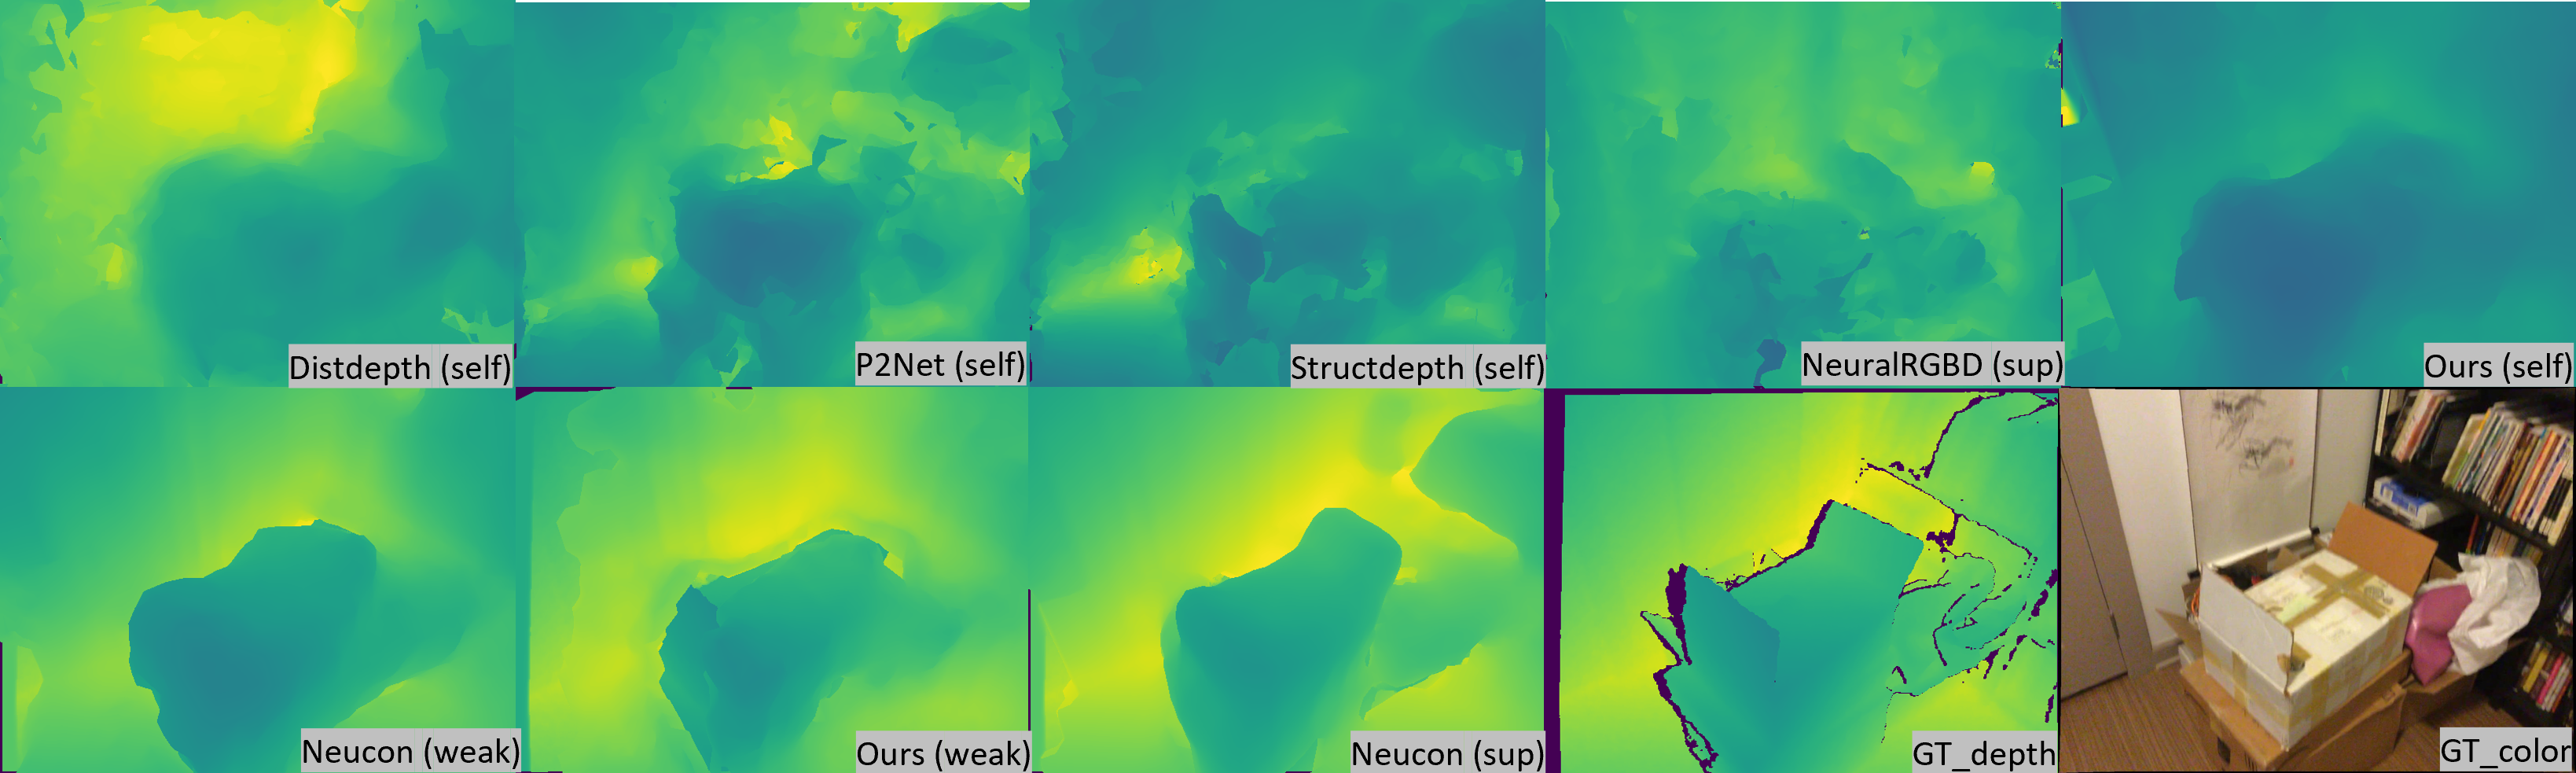
\includegraphics[width=1.0\textwidth]{figures/scannet_depth/710_1280.png}}
\end{minipage}
%\vspace{-3mm}
\begin{minipage}{\linewidth}
  \centerline{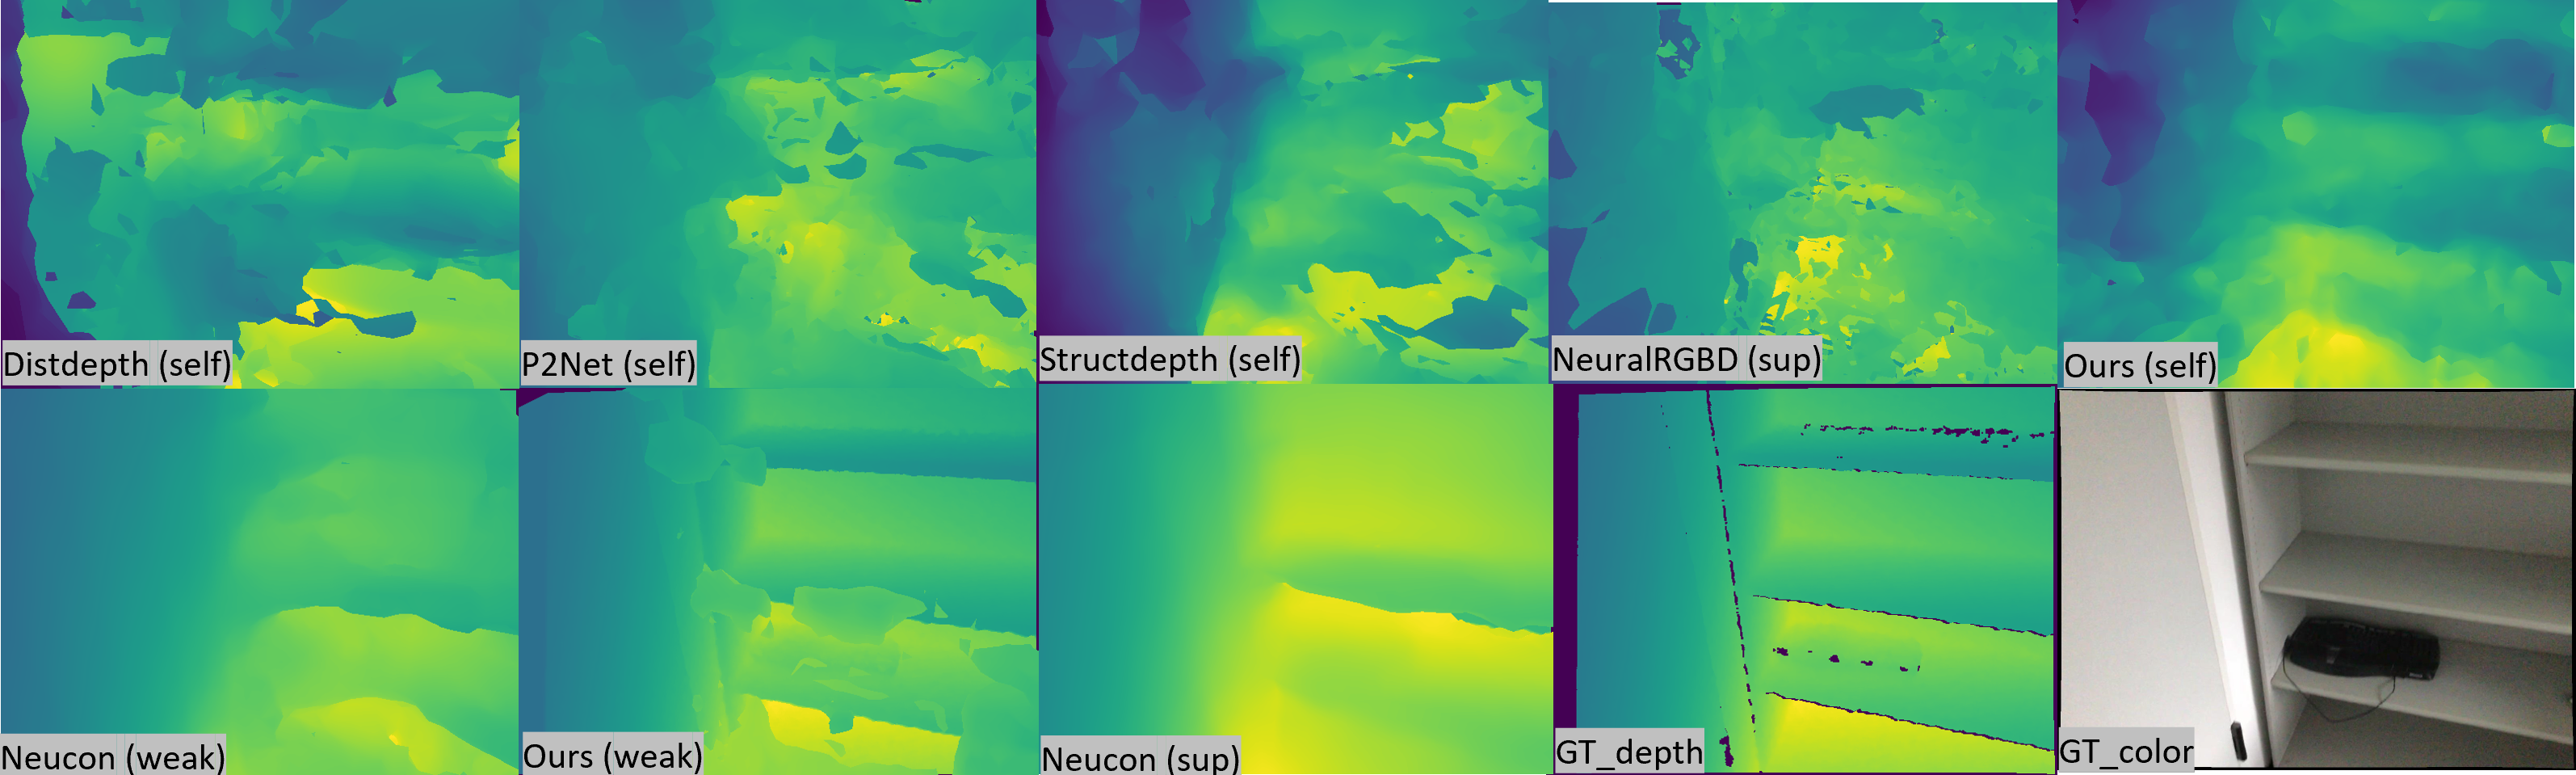
\includegraphics[width=1.0\textwidth]{figures/scannet_depth/711_880.png}}
\end{minipage}
%\vspace{-3mm}
\end{figure*}

\newpage
\begin{figure*}
\begin{minipage}{\textwidth}
  \centerline{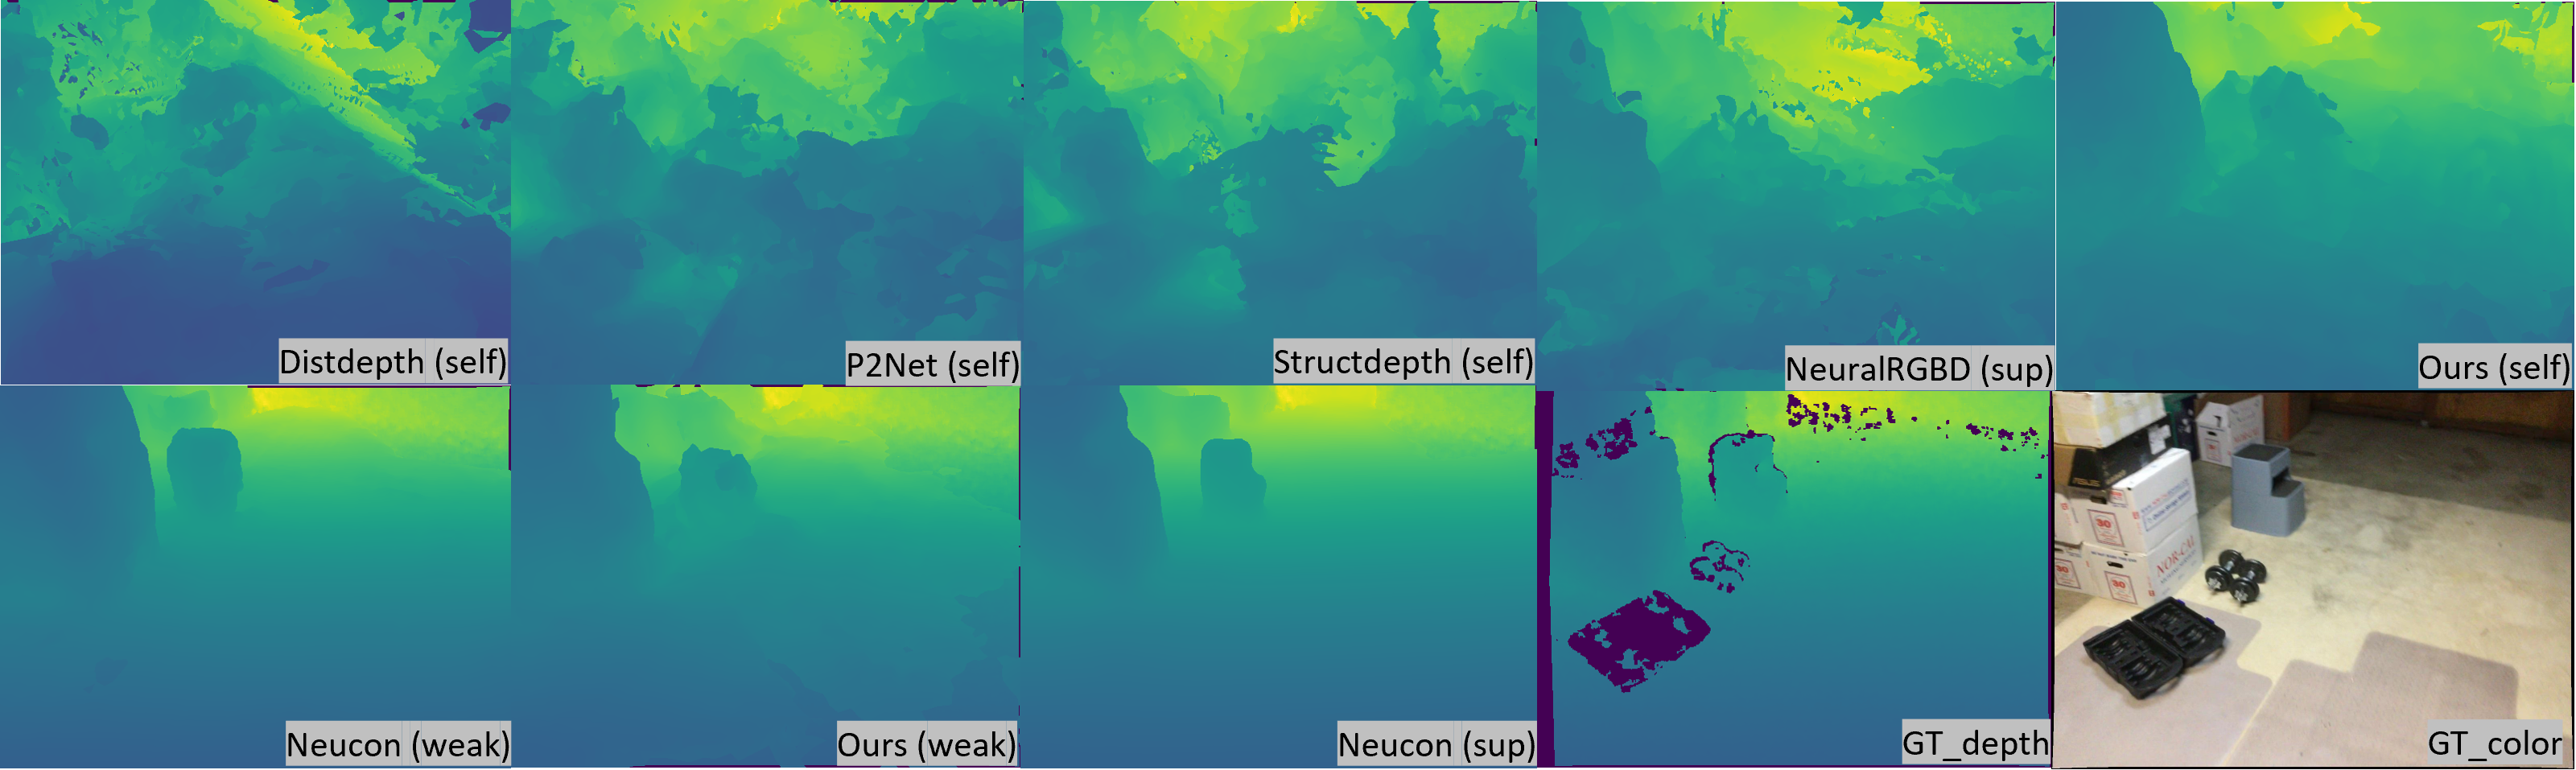
\includegraphics[width=1.0\textwidth]{figures/scannet_depth/787_1720.png}}
\end{minipage}
\vfill
\begin{minipage}{\linewidth}
  \centerline{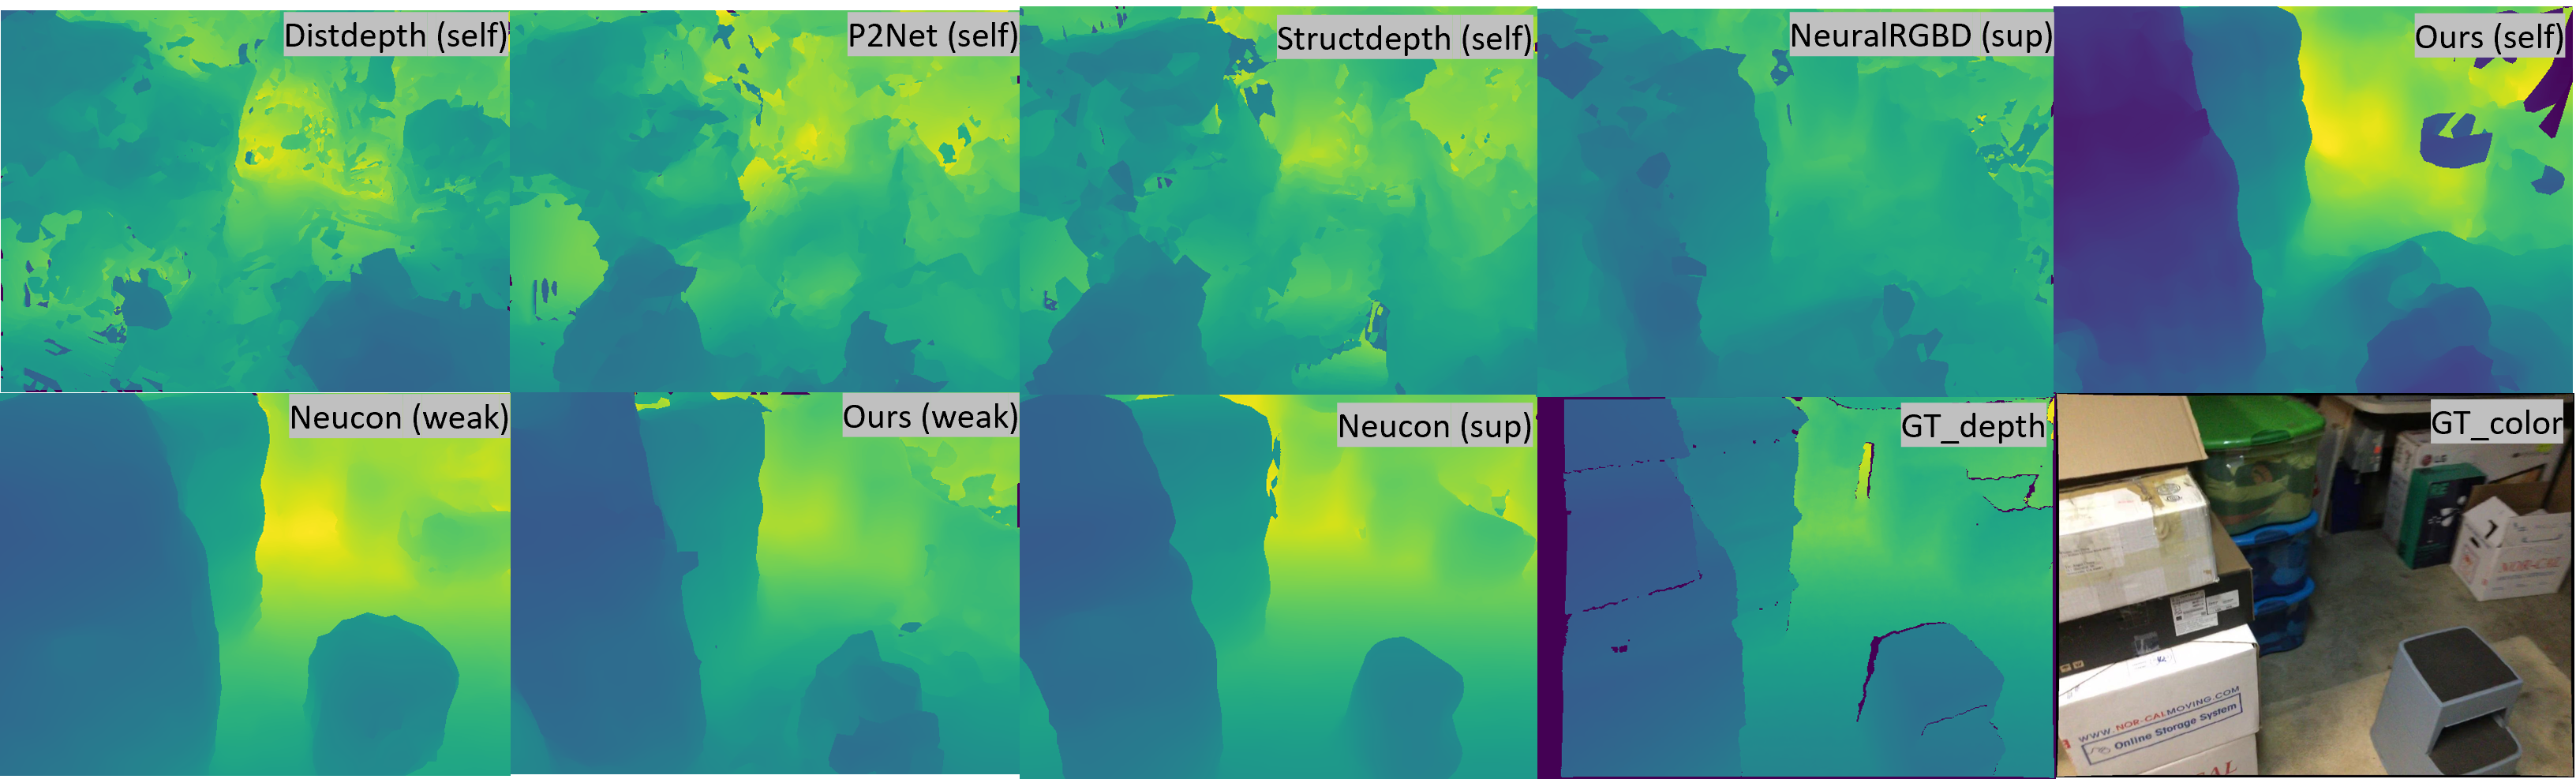
\includegraphics[width=1.0\textwidth]{figures/scannet_depth/787_1930.png}}
\end{minipage}
\vfill
\begin{minipage}{\linewidth}
  \centerline{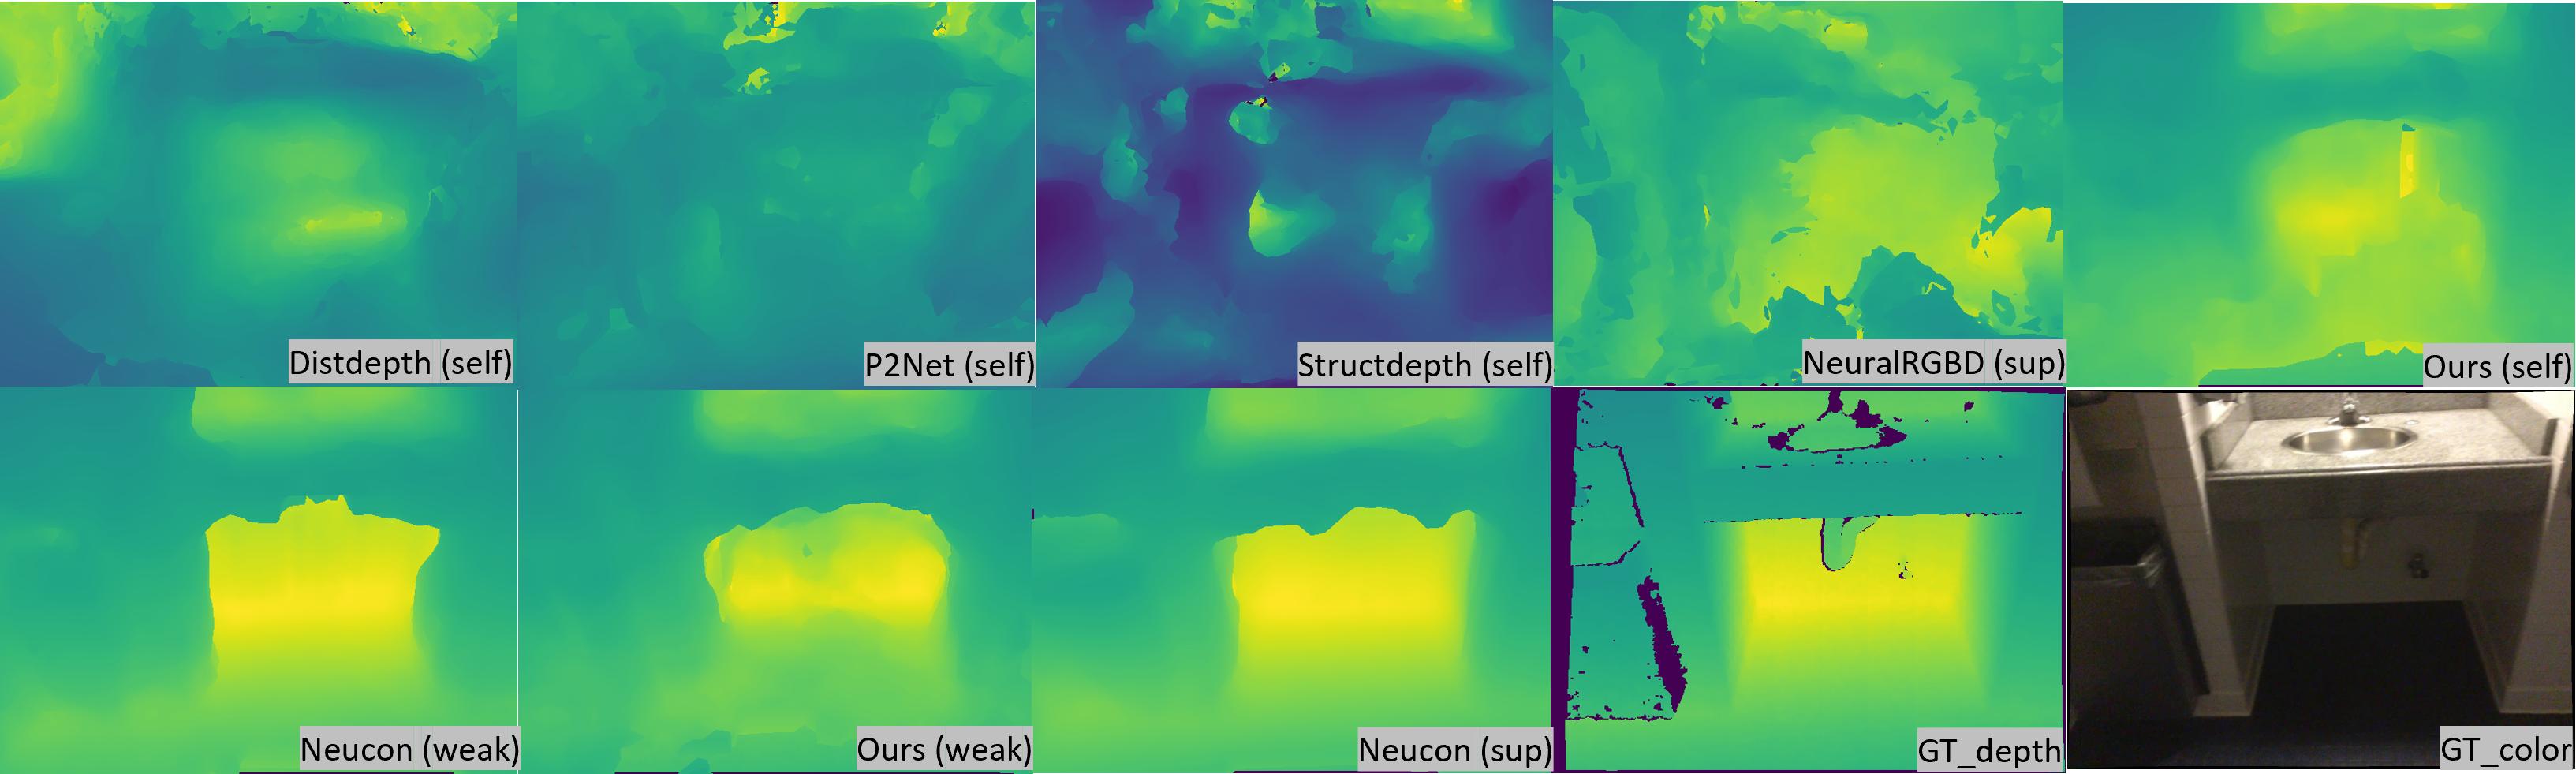
\includegraphics[width=1.0\textwidth]{figures/scannet_depth/779_1125.png}}
\end{minipage}
%\vspace{-3mm}
\begin{minipage}{\linewidth}
  \centerline{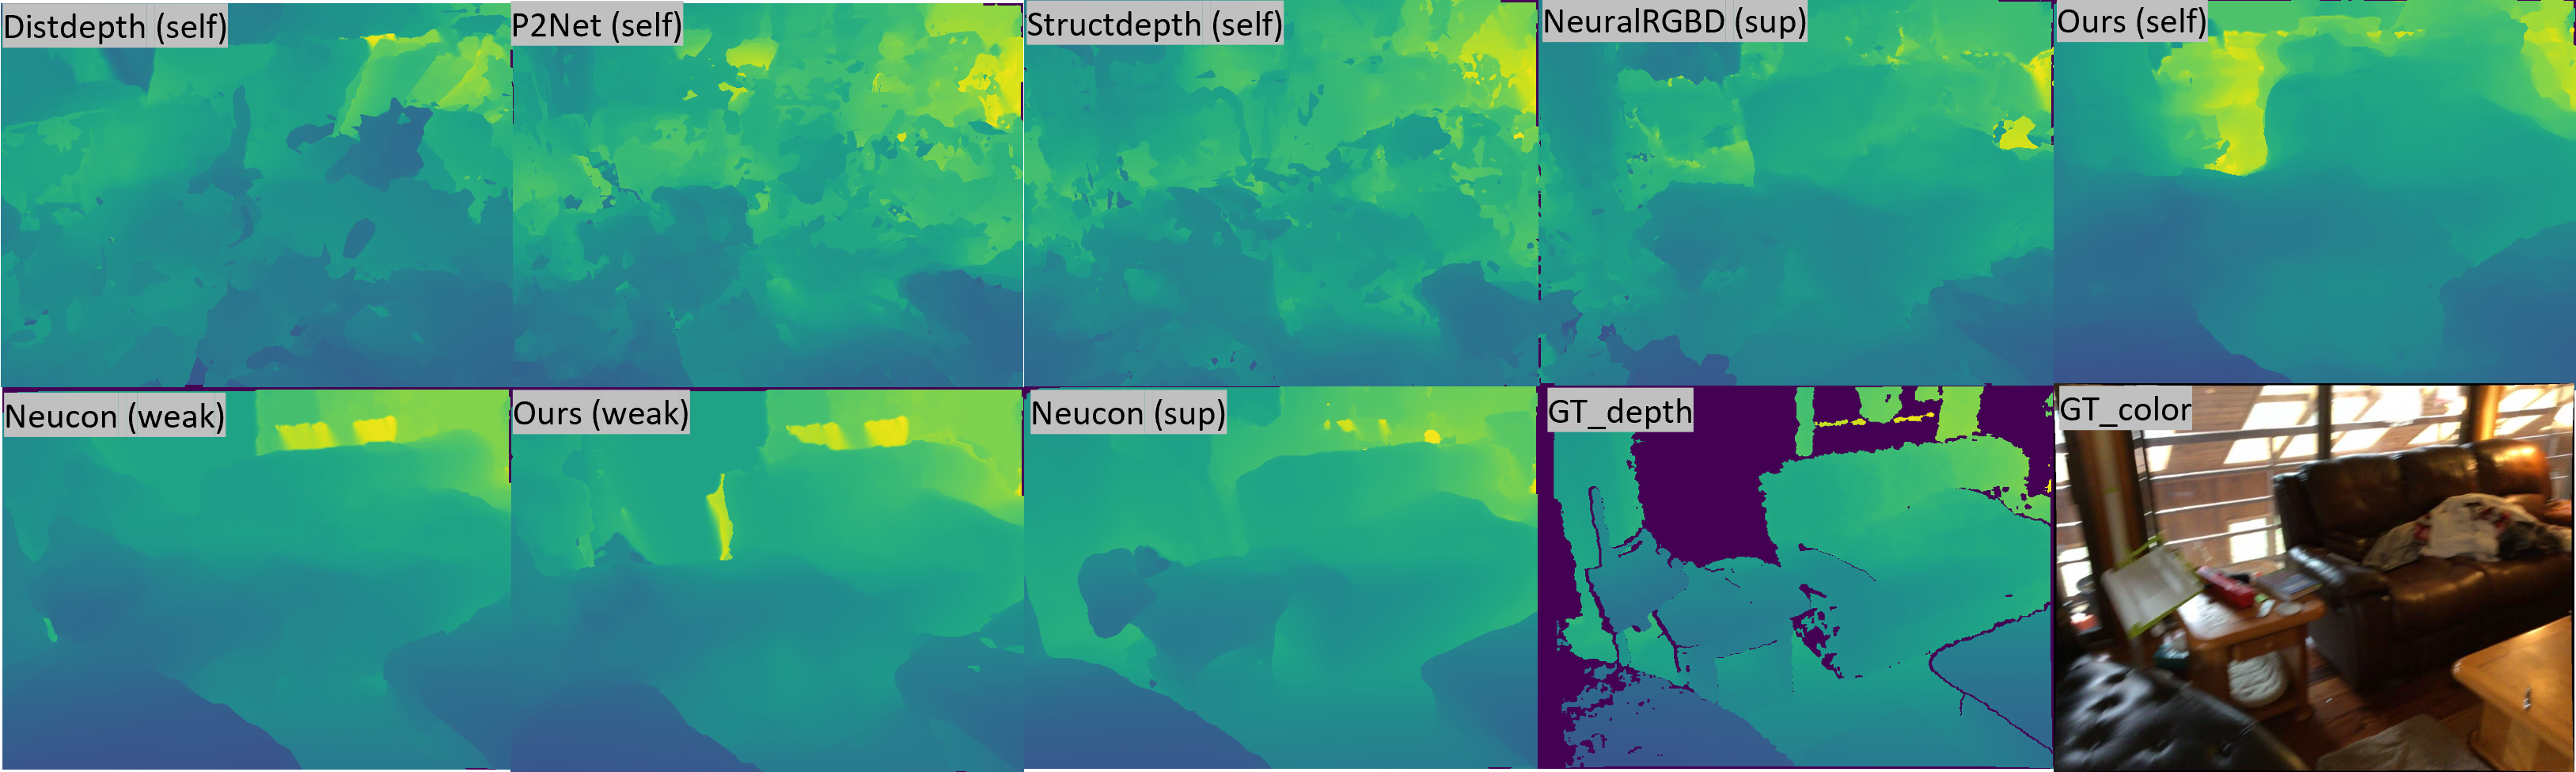
\includegraphics[width=1.0\textwidth]{figures/scannet_depth/747_97.png}}
\end{minipage}
%\vspace{-3mm}
\vspace{-3mm}
\end{figure*}

\newpage
\begin{figure*}
\begin{minipage}{\textwidth}
  \centerline{\includegraphics[width=1.0\textwidth]{figures/scannet_mesh/787.png}}
\end{minipage}
\vfill
\begin{minipage}{\linewidth}
  \centerline{\includegraphics[width=1.0\textwidth]{figures/scannet_mesh/747.png}}
\end{minipage}

\iffalse
\vfill
\begin{minipage}{\linewidth}
  \centerline{\includegraphics[width=1.0\textwidth]{figures/scannet_mesh/710.png}}
\end{minipage}
\fi
\label{fig:scannet_supp}
    \caption{Visual Results}
\end{figure*}


\end{document}
